%!TEX ROOT = main.tex

\section{Lab 3}

Nim is a simple game where two players take turns removing objects from a pile. The player who removes the last object wins. The game is described in detail here. There is a mathematical strategy to win Nim, by ensuring you always leave the opponent with a nim-sum number of objects (groups of 1, 2 and 4).

In this notebook, we will play nim-sum using the following agents:

\begin{enumerate}
    \item An agent using fixed rules based on nim-sum
    \item An agent using evolved rules
    \item An agent using minmax
    \item An agent using reinforcement learning (both temporal difference learning and monte carlo learning)
\end{enumerate}


\subsection{Solution}

\subsubsection{Fixed Rules}

I came up with multiple rules, through discussion with friends and through research papers that define fixed rules for playing Nim. There are currently 4 rules implemented. The rules are as follows:

\begin{enumerate}
    \item If one pile, take x number of sticks from the pile.
    \item If two piles, take x number of sticks from the larger pile.
    \item If two piles: a. If 1 pile has 1 stick, take x sticks b. If 2 piles have multiple sticks, take x sticks from the larger pile
    \item If three piles and two piles have the same size, remove all sticks from the smallest pile
    \item If n piles and n-1 piles have the same size, remove x sticks from the smallest pile until it is the same size as the other piles
\end{enumerate}

\begin{figure}
    \centering
    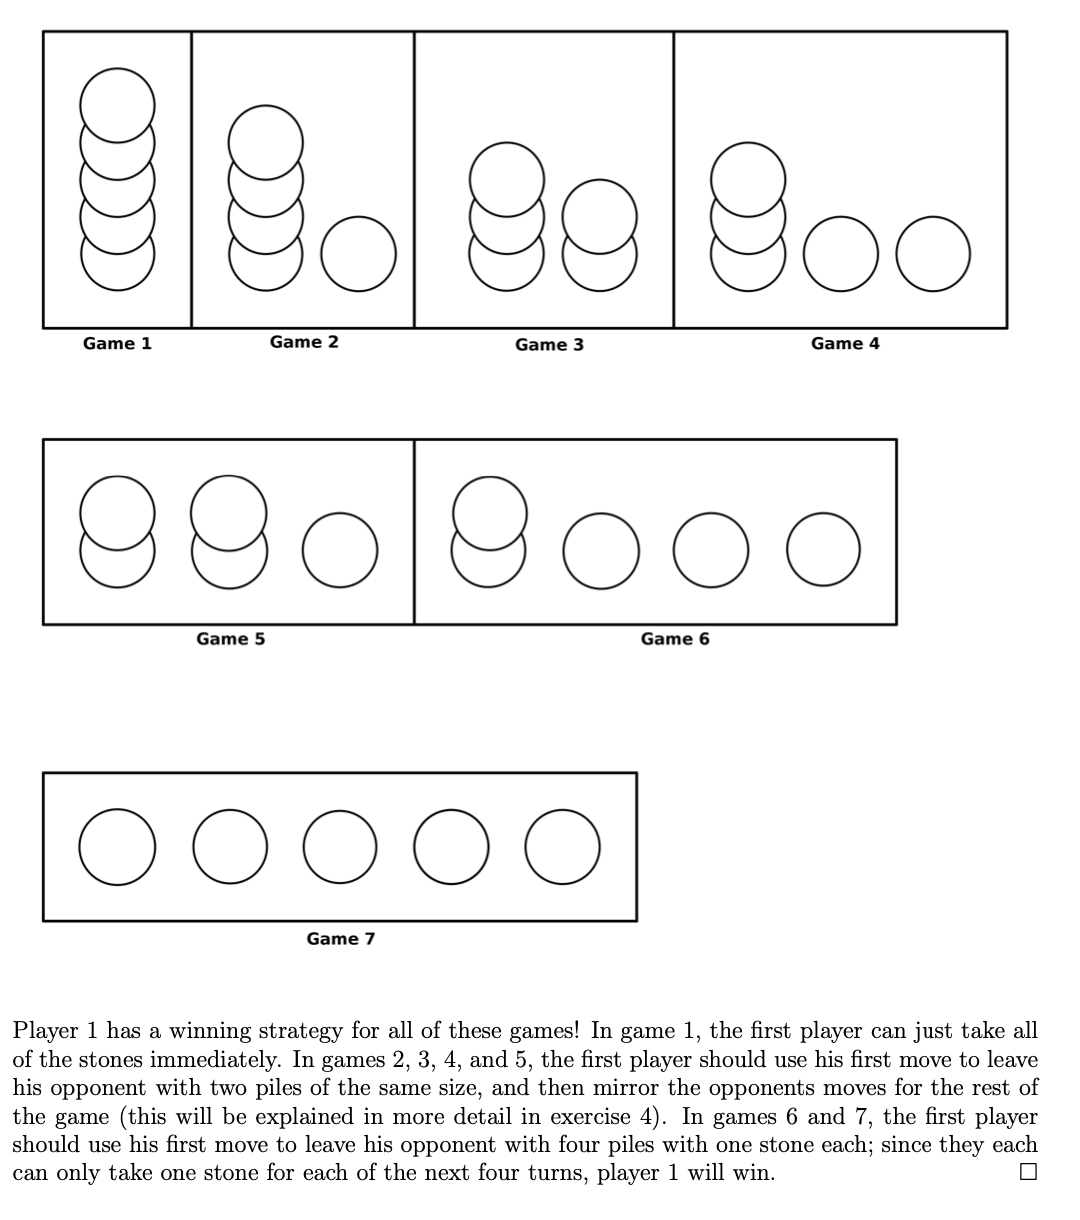
\includegraphics[width=0.5\textwidth]{images/rules.png}
    \caption{Fixed Rules}
    \label{fig:fixed_rules}
\end{figure}


\paragraph{Approach 1: A Lot of If-Elses}
The above rules are applied directly. An if-else sequence decides which strategy to employ based on the current layout and statistics on the nim board.

\begin{mintedbox}{python}
    from collections import Counter
    from copy import deepcopy
    from itertools import accumulate
    import logging
    from operator import xor
    import random
    from typing import Callable

    from lib import Genome, Nim, Nimply


    class FixedRuleNim:
        def __init__(self):
            self.num_moves = 0
            self.OFFSPRING_SIZE = 30
            self.POPULATION_SIZE = 100
            self.GENERATIONS = 100
            self.nim_size = 5

        def nim_sum(self, nim: Nim):
            '''
            Returns the nim sum of the current game board
            by taking an XOR of all the rows.
            Ideally, agent should try to leave nim sum of 0 at the end of turn
            '''
            *_, result = accumulate(nim.rows, xor)
            return result

        def init_population(self, population_size, nim: Nim):
            '''
            Initialize population of genomes,
            key is rule, value is number of sticks to take
            The rules currently are:
            1. If one pile, take $x$ number of sticks from the pile.
            2. If two piles:
                a. If 1 pile has 1 stick, wipe out the pile
                b. If 2 piles have multiple sticks, take x sticks from any pile
            3. If three piles and two piles have the same size, remove all sticks from the smallest pile
            4. If n piles and n-1 piles have the same size, remove x sticks from the smallest pile until it is the same size as the other piles
            '''
            population = []
            for i in range(population_size):
                # rules 3 and 4 are fixed (apply for 3 or more piles)
                # different strategies for different rules (situations on the board)
                individual = {
                    'rule_1': [0, random.randint(0, (nim.num_rows - 1) * 2)],
                    'rule_2a': [random.randint(0, 1), random.randint(0, (nim.num_rows - 1) * 2)],
                    'rule_2b': [random.randint(0, 1), random.randint(0, (nim.num_rows - 1) * 2)],
                    'rule_3': [nim.rows.index(min(nim.rows)), min(nim.rows)],
                    'rule_4': [nim.rows.index(max(nim.rows)), max(nim.rows) - min(nim.rows)]
                }
                genome = Genome(individual)
                population.append(genome)
            return population

        def statistics(self, nim: Nim):
            '''
            Similar to Squillero's cooked function to get possible moves
            and statistics on Nim board
            '''
            # logging.info('In statistics')
            # logging.info(nim.rows)
            stats = {
                'possible_moves': [(r, o) for r, c in enumerate(nim.rows) for o in range(1, c + 1) if nim.k is None or o <= nim.k],
                # 'possible_moves': [(row, num_objects) for row in range(nim.num_rows) for num_objects in range(1, nim.rows[row]+1)],
                'num_active_rows': sum(o > 0 for o in nim.rows),
                'shortest_row': min((x for x in enumerate(nim.rows) if x[1] > 0), key=lambda y: y[1])[0],
                'longest_row': max((x for x in enumerate(nim.rows)), key=lambda y: y[1])[0],
                # only 1-stick row and not all rows having only 1 stick
                '1_stick_row': any([1 for x in nim.rows if x == 1]) and not all([1 for x in nim.rows if x == 1]),
                'nim_sum': self.nim_sum(nim)
            }

            brute_force = []
            for move in stats['possible_moves']:
                tmp = deepcopy(nim)
                tmp.nimming_remove(*move)
                brute_force.append((move, self.nim_sum(tmp)))
            stats['brute_force'] = brute_force

            return stats

        def strategy(self):
            '''
            Returns the best move to make based on the statistics
            '''
            def engine(nim: Nim):
                stats = self.statistics(nim)
                if stats['num_active_rows'] == 1:
                    # logging.info('m1')
                    return Nimply(stats['shortest_row'], random.randint(1, stats['possible_moves'][0][1]))
                elif stats["num_active_rows"] % 2 == 0:
                    # logging.info('m2')
                    if max(nim.rows) == 1:
                        return Nimply(stats['longest_row'], 1)
                    else:
                        pile = random.choice([i for i, x in enumerate(nim.rows) if x > 1])
                        return Nimply(pile, nim.rows[pile] - 1)
                elif stats['num_active_rows'] == 3:
                    # logging.info('m3')
                    unique_elements = set(nim.rows)
                    # check if 2 rows have the same number of sticks
                    two_rows_with_same_elements = False
                    for element in unique_elements:
                        if nim.rows.count(element) == 2:
                            two_rows_with_same_elements = True
                            break

                    if len(nim.rows) == 3 and two_rows_with_same_elements:
                        # remove 1 stick from the longest row
                        logging.info(nim.rows)
                        return Nimply(stats['longest_row'], max(max(nim.rows) - nim.rows[stats['shortest_row']], 1))
                    else:
                        # do something random
                        return Nimply(*random.choice(stats['possible_moves']))
                elif stats['num_active_rows'] >= 4:
                    # logging.info('m4')
                    counter = Counter()
                    for element in nim.rows:
                        counter[element] += 1
                    if len(counter) == 2:
                        if counter.most_common()[0][1] == 1:
                            # remove x sticks from the smallest pile until it is the same size as the other piles
                            return Nimply(stats['shortest_row'], max(nim.rows[stats['shortest_row']] - counter.most_common()[1][0], 1))
                    return random.choice(stats['possible_moves'])
                else:
                    # logging.info('m5')
                    return random.choice(stats['possible_moves'])
            return engine

        def random_agent(self, nim: Nim):
            '''
            Random agent that takes a random move
            '''
            stats = self.statistics(nim)
            return random.choice(stats['possible_moves'])

        def battle(self, opponent, num_games=1000):
            '''
            Battle this agent against another agent
            '''
            wins = 0
            for _ in range(num_games):
                nim = Nim()
                while not nim.goal():
                    nim.nimming_remove(*self.play(nim))
                    if sum(nim.rows) == 0:
                        break
                    nim.nimming_remove(*opponent.play(nim))
                if sum(nim.rows) == 0:
                    wins += 1
            return wins

    if __name__ == '__main__':
        rounds = 20
        evolved_agent_wins = 0
        for i in range(rounds):
            nim = Nim(5)
            orig = nim.rows
            fixedrule = FixedRuleNim()
            engine = fixedrule.strategy()

            # play against random
            player = 0
            while not nim.goal():
                if player == 0:
                    move = engine(nim)
                    logging.info('move of player 1: ', move)
                    nim.nimming_remove(*move)
                    player = 1
                    logging.info("After Player 1 made move: ", nim.rows)
                else:
                    move = fixedrule.random_agent(nim)
                    logging.info('move of player 2: ', move)
                    nim.nimming_remove(*move)
                    player = 0
                    logging.info("After Player 2 made move: ", nim.rows)
            winner = 1 - player
            if winner == 0:
                evolved_agent_wins += 1
        logging.info(f'Fixed rule agent won {evolved_agent_wins} out of {rounds} games')
\end{mintedbox}

\paragraph{Approach 2: Nim-Sum} Will always win
\begin{mintedbox}{python}
from copy import deepcopy
from itertools import accumulate
from operator import xor
import random
import logging
from lib import Nim

# 3.1: Agent Using Fixed Rules
class ExpertNimSumAgent:
    '''
    Play the game of Nim using a fixed rule
    (always leave nim-sum at the end of turn)
    '''
    def __init__(self):
        self.num_moves = 0

    def nim_sum(self, nim: Nim):
        '''
        Returns the nim sum of the current game board
        by taking an XOR of all the rows.
        Ideally, agent should try to leave nim sum of 0 at the end of turn
        '''
        *_, result = accumulate(nim.rows, xor)
        return result
        # return sum([i^r for i, r in enumerate(nim._rows)])

    def play(self, nim: Nim):
        # remove objects from row to make nim-sum 0
        nim_sum = self.nim_sum(nim)
        all_possible_moves = [(r, o) for r, c in enumerate(nim.rows) for o in range(1, c+1)]
        move_found = False
        for move in all_possible_moves:
            replicated_nim = deepcopy(nim)
            replicated_nim.nimming_remove(*move)
            if self.nim_sum(replicated_nim) == 0:
                nim.nimming_remove(*move)
                move_found = True
                break
        # if a valid move not found, return random move
        if not move_found:
            move = random.choice(all_possible_moves)
            nim.nimming_remove(*move)

        # logging.info(f"Move {self.num_moves}: Removed {move[1]} objects from row {move[0]}")
        self.num_moves += 1
\end{mintedbox}

\subsubsection{Evolved Agent Approach 1}

The rules are evolved using a genetic algorithm. A dictionary of strategies is evolved. The key is the rule (scenario/antecedent). The value is the maximum number of sticks to leave on the board in this scenario.

For instance, for rule 1, the value tuned is the
 in "If one pile, leave a max of x sticks in the pile".

\begin{markdown}
    rule_strategy = {
        "one_pile": 2,
        "two_piles": 3,
        "three_piles": 3,
        "n_piles": 4
    }

    # after mutation / crossover
    rule_strategy = {
        "one_pile": 3,
        "two_piles": 2,
        "three_piles": 3,
        "n_piles": 4
    }

\end{markdown}

Mutation essentially swaps the values in the dictionaries. Crossover takes two parents and randomly chooses strategies for different rules. Intuitively, the machine tries to learn the best strategy for each scenario on the board.

\begin{table}
\centering
\begin{tabular}{|c|c|c|}
\hline
Opponent 1 & Opponent 2 & Win Rate \\ \hline
Evolved & Random & 70\% \\ \hline
\end{tabular}
\end{table}

\begin{mintedbox}{python}
    '''
In this file, I will try to implement Nim where there is an evolved set of rules/strategies.
For each scenario, I will have a set of rules that will be used to determine the best move.
They are obtained from discussion with friends and from the paper "The Game of Nim" by Ryan Julian
The rules currently are:
1. If one pile, take $x$ number of sticks from the pile.
2. If two piles:
    a. If 1 pile has 1 stick, take x sticks
    b. If 2 piles have multiple sticks, take x sticks from the larger pile
3. If three piles and two piles have the same size, remove all sticks from the smallest pile
4. If n piles and n-1 piles have the same size, remove x sticks from the smallest pile until it is the same size as the other piles
'''

from collections import Counter, namedtuple
from copy import deepcopy
from itertools import accumulate
import logging
from operator import xor
import random
from typing import Callable

from lib import Genome, Nim, Nimply

class BrilliantEvolvedAgent:
    def __init__(self):
        self.num_moves = 0
        self.OFFSPRING_SIZE = 200
        self.POPULATION_SIZE = 50
        self.GENERATIONS = 100
        self.nim_size = 5

    def nim_sum(self, nim: Nim):
        '''
        Returns the nim sum of the current game board
        by taking an XOR of all the rows.
        Ideally, agent should try to leave nim sum of 0 at the end of turn
        '''
        *_, result = accumulate(nim.rows, xor)
        return result

    def init_population(self, population_size, nim: Nim):
        '''
        Initialize population of genomes,
        key is rule, value is number of sticks to take
        The rules currently are:
        1. If one pile, take $x$ number of sticks from the pile.
        2. If two piles:
            a. If 1 pile has 1 stick, wipe out the pile
            b. If 2 piles have multiple sticks, take x sticks from any pile
        3. If three piles and two piles have the same size, remove all sticks from the smallest pile
        4. If n piles and n-1 piles have the same size, remove x sticks from the smallest pile until it is the same size as the other piles
        5. If none of the above rules apply, just pick a random pile and take a random number of sticks
        '''
        population = []
        for i in range(population_size):
            # rules 3 and 4 are fixed (apply for 3 or more piles)
            # different strategies for different rules (situations on the board)
            individual = {
                'rule_1': [0, random.randint(0, (self.nim_size - 1) * 2)],
                'rule_2a': [random.randint(0, 1), random.randint(0, (self.nim_size - 1) * 2)],
                'rule_2b': [random.randint(0, 1), random.randint(0, (self.nim_size - 1) * 2)],
                'rule_3': [nim.rows.index(min(nim.rows)), min(nim.rows)],
                'rule_4': [nim.rows.index(max(nim.rows)), max(nim.rows) - min(nim.rows)]
            }
            genome = Genome(individual)
            population.append(genome)
        return population

    def crossover(self, parent1, parent2, crossover_rate):
        '''
        Crossover function to combine two parents into a child
        '''
        child = {}
        for rule in parent1.rules:
            if random.random() < crossover_rate:
                child[rule] = parent1.rules[rule]
            else:
                child[rule] = parent2.rules[rule]
        return Genome(child)

    def tournament_selection(self, population, tournament_size):
        '''
        Tournament selection to select the best genomes
        '''
        tournament = random.sample(population, tournament_size)
        tournament.sort(key=lambda x: x.fitness, reverse=True)
        return tournament[0]

    def mutate(self, genome: Genome, mutation_rate=0.5):
        '''
        Mutate the genome by switching one of the rules (can end up in something stupid like removing more sticks than there are, but this is checked in the strategy function)
        '''
        rule = random.choice(list(genome.rules.keys()))
        # swap some keys
        if rule == 'rule_1':
            genome.rules[rule] = [0, random.randint(0, (self.nim_size - 1) * 2)]
        elif rule == 'rule_2a':
            genome.rules[rule] = [random.randint(0, 1), random.randint(0, (self.nim_size - 1) * 2)]
        elif rule == 'rule_2b':
            genome.rules[rule] = [random.randint(0, 1), random.randint(0, (self.nim_size - 1) * 2)]
        elif rule == 'rule_3':
            genome.rules[rule] = [random.randint(0, self.nim_size - 1), random.randint(0, (self.nim_size - 1) * 2)]
        elif rule == 'rule_4':
            genome.rules[rule] = [random.randint(0, self.nim_size - 1), random.randint(0, (self.nim_size - 1) * 2)]
        return genome
        # rule = random.choice(list(genome.rules.keys()))
        # if random.random() < mutation_rate:
        #     genome.rules[rule] = [random.randint(0, 1), random.randint(0, self.nim_size * 2)]
        # return genome
        # rule = random.choice(list(genome.keys()))
        # genome[rule] = random.randint(1, 10)

    def statistics(self, nim: Nim):
        '''
        Similar to Squillero's cooked function to get possible moves
        and statistics on Nim board
        '''
        stats = {
            'possible_moves': [(r, o) for r, c in enumerate(nim.rows) for o in range(1, c + 1) if nim.k is None or o <= nim.k],
            # 'possible_moves': [(row, num_objects) for row in range(nim.num_rows) for num_objects in range(1, nim.rows[row]+1)],
            'num_active_rows': sum(o > 0 for o in nim.rows),
            'shortest_row': min((x for x in enumerate(nim.rows) if x[1] > 0), key=lambda y: y[1])[0],
            'longest_row': max((x for x in enumerate(nim.rows)), key=lambda y: y[1])[0],
            # only 1-stick row and not all rows having only 1 stick
            '1_stick_row': any([1 for x in nim.rows if x == 1]) and not all([1 for x in nim.rows if x == 1]),
            'nim_sum': self.nim_sum(nim)
        }

        brute_force = []
        for move in stats['possible_moves']:
            tmp = deepcopy(nim)
            tmp.nimming_remove(*move)
            brute_force.append((move, self.nim_sum(tmp)))
        stats['brute_force'] = brute_force

        return stats

    def strategy(self, genome: dict):
        '''
        Returns the best move to make based on the statistics
        '''
        def evolution(nim: Nim):
            stats = self.statistics(nim)
            if stats['num_active_rows'] == 1:
                num_to_leave = genome.rules['rule_1'][1]
                # see which move will leave the most sticks
                most_destructive_move = max(stats['possible_moves'], key=lambda x: x[1])
                if num_to_leave >= most_destructive_move[1]:
                    # remove only 1 stick
                    return Nimply(most_destructive_move[0], 1)
                else:
                    # make the move that leaves the desired number of sticks
                    move = [(row, num_objects) for row, num_objects in stats['possible_moves'] if nim.rows[row] - num_objects == num_to_leave]
                    if len(move) > 0:
                        return Nimply(*move[0])
                    else:
                        # make random move
                        return Nimply(*random.choice(stats['possible_moves']))

            elif stats['num_active_rows'] == 2:
                # rule 2a
                if stats['1_stick_row']:
                    # if there is a 1-stick row, have to choose between wiping it out or taking from the other row
                    if genome.rules['rule_2a'][0] == 0:
                        # wipe out the 1-stick row
                        logging.info('wiping out 1-stick row')
                        pile = [row for row in range(nim.num_rows) if nim.rows[row] == 1][0]
                        return Nimply(pile, 1)
                    else:
                        # take out the desired number of sticks from the other row
                        pile = random.choice([index for index, x in enumerate(nim.rows) if x > 1])
                        num_objects_to_remove = max(1, nim.rows[pile] - genome.rules['rule_2a'][1])
                        # move = [(row, num_objects) for row, num_objects in stats['possible_moves'] if nim.rows[row] - num_objects == genome.rules['rule_2a'][1]]
                        return Nimply(pile, num_objects_to_remove)
                # rule 2b
                # both piles have many elements, take from either the smallest or the largest pile
                else:
                    if genome.rules['rule_2b'][0] == 0:
                        # take from the smallest pile
                        pile = stats['shortest_row']
                        num_objects_to_remove = max(1, nim.rows[pile] - genome.rules['rule_2b'][1])
                        return Nimply(pile, num_objects_to_remove)
                    else:
                        # take from the largest pile
                        pile = stats['longest_row']
                        num_objects_to_remove = max(1, nim.rows[pile] - genome.rules['rule_2b'][1])
                        return Nimply(pile, num_objects_to_remove)

            elif stats['num_active_rows'] == 3:
                unique_elements = set(nim.rows)
                # check if 2 rows have the same number of sticks
                two_rows_with_same_elements = False
                for element in unique_elements:
                    if nim.rows.count(element) == 2:
                        two_rows_with_same_elements = True
                        break

                if len(nim.rows) == 3 and two_rows_with_same_elements:
                    # remove 1 stick from the longest row
                    return Nimply(stats['longest_row'], max(max(nim.rows) - nim.rows[stats['shortest_row']], 1))
                else:
                    # do something random
                    return Nimply(*random.choice(stats['possible_moves']))

            counter = Counter()
            for element in nim.rows:
                counter[element] += 1
            if len(counter) == 2:
                if counter.most_common()[0][1] == 1:
                    # remove x sticks from the smallest pile until it is the same size as the other piles
                    return Nimply(stats['shortest_row'], max(nim.rows[stats['shortest_row']] - counter.most_common()[1][0], 1))
                # else:
                #     return random.choice(stats['possible_moves'])

            # for large number of piles, general rule to remove all but 1 stick from a random pile
            if stats["num_active_rows"] % 2 == 0:
                if nim.rows[stats['longest_row']] == 1:
                    return Nimply(stats['longest_row'], 1)
                else:
                    pile = random.choice([i for i, x in enumerate(nim.rows) if x > 1])
                    return Nimply(pile, nim.rows[pile] - 1)

            else:
                # this is a fixed rule, does not have random component
                # rule from the paper Ryan Julian: The Game of Nim
                # If n piles and n-1 piles have the same size, remove x sticks from the smallest pile until it is the same size as the other piles
                # check if only 1 pile has a different number of sticks
                # just make a random move if all else fails
                return random.choice(stats['possible_moves'])
        return evolution

    def random_agent(self, nim: Nim):
        '''
        Random agent that takes a random move
        '''
        stats = self.statistics(nim)
        return random.choice(stats['possible_moves'])

    def dumb_agent(self, nim: Nim):
        '''
        Agent that takes one element from the longest row
        '''
        stats = self.statistics(nim)
        return (stats['longest_row'], 1)

    def aggressive_agent(self, nim: Nim):
        '''
        Agent that takes the largest possible move
        '''
        stats = self.statistics(nim)
        if stats['num_active_rows'] % 2 == 0:
            return random.choice(stats['possible_moves'])
        else:
            row = stats['longest_row']
            return (row, nim.rows[row])

        # stats = self.statistics(nim)
        # return max(stats['possible_moves'], key=lambda x: x[1])

    def calculate_fitness(self, genome):
        '''
        Calculate fitness by playing the genome's strategy against a random agent
        (cannot use nim sum agent as it is too good)
        '''
        wins = 0
        for i in range(5):
            nim = Nim(5)
            player = 0
            engine = self.strategy(genome)
            while not nim.goal():
                if player == 0:
                    move = engine(nim)
                    nim.nimming_remove(*move)
                    player = 1
                else:
                    nim.nimming_remove(*self.random_agent(nim))
                    player = 0
            winner = 1 - player
            if winner == 0:
                wins += 1
        return wins / 5

    def select_survivors(self, population: list, num_survivors: int):
        '''
        Select the best genomes from the population
        '''
        return sorted(population, key=lambda x: x.fitness, reverse=True)[:num_survivors]

    def learn(self, population_size=100, mutation_rate=0.1, crossover_rate=0.7, nim: Nim = None):
        initial_population = self.init_population(population_size, nim)
        for genome in initial_population:
            genome.fitness = self.calculate_fitness(genome)
        for i in range(self.GENERATIONS):
            # logging.info(f'Generation {i}')
            new_offspring = []
            for j in range(self.OFFSPRING_SIZE):
                parent1 = random.choice(initial_population)
                parent2 = random.choice(initial_population)
                child = self.crossover(parent1, parent2, crossover_rate)
                child = self.mutate(child)
                new_offspring.append(child)
            initial_population += new_offspring
            initial_population = self.select_survivors(initial_population, population_size)
        best_strategy = initial_population[0]
        return best_strategy

    def battle(self, opponent, num_games=1000):
        '''
        Battle this agent against another agent
        '''
        wins = 0
        for _ in range(num_games):
            nim = Nim()
            while not nim.goal():
                nim.nimming_remove(*self.play(nim))
                if sum(nim.rows) == 0:
                    break
                nim.nimming_remove(*opponent.play(nim))
            if sum(nim.rows) == 0:
                wins += 1
        return wins

if __name__ == '__main__':
    rounds = 20
    evolved_agent_wins = 0
    for i in range(rounds):
        nim = Nim(5)
        orig = nim.rows
        brilliantagent = BrilliantEvolvedAgent()
        best_strategy = brilliantagent.learn(nim=nim)
        engine = brilliantagent.strategy(best_strategy)

        # play against random
        player = 0
        while not nim.goal():
            if player == 0:
                move = engine(nim)
                logging.info('move of player 1: ', move)
                nim.nimming_remove(*move)
                player = 1
                logging.info("After Player 1 made move: ", nim.rows)
            else:
                move = brilliantagent.random_agent(nim)
                logging.info('move of player 2: ', move)
                nim.nimming_remove(*move)
                player = 0
                logging.info("After Player 2 made move: ", nim.rows)
        winner = 1 - player
        if winner == 0:
            evolved_agent_wins += 1
    logging.info(f'Evolved agent won {evolved_agent_wins} out of {rounds} games')
\end{mintedbox}

\subsubsection{Evolved Agent Approach 2 (Probability Thresholds)}

Strategies were originally chosen based on probability thresholds and a random number. The list of probabilities (thresholds) are evolved using a genetic algorithm. \emph{Intuitively, the machine tries to learn the best probability of choosing each strategy, regardless of the rule.}

\begin{mintedbox}{python}
    thresholds = [p1, p2, p3]
    if random.random() < p1:
        # strategy 1...
    elif random.random() < p2:
        # strategy 2...
    else:
        # strategy 3...

    class GA:
        ...

    GA.evolve(thresholds)
\end{mintedbox}

I discussed this approach with both Prof. Squillero and Calabrese. They both agreed that this was worth exploring. However, upon implementing, I realised that tuning probability thresholds produces poor, near-random performance, \emph{as the system is making decisions without any knowledge of the current situation on the board, or any knowledge of the rules}.

\begin{mintedbox}{python}
    # 3.2: Agent Using Evolved Rules (Randomly Chooses Between Strategies Based on Probabilities)
    from itertools import accumulate
    from operator import xor
    import random
    import numpy as np

    from lib import Nim

    class EvolvedAgent1:
        '''
        Plays Nim using a set of rules that are evolved
        '''
        def __init__(self):
            self.num_moves = 0

        def nim_sum(self, nim: Nim):
            '''
            Returns the nim sum of the current game board
            by taking an XOR of all the rows.
            Ideally, agent should try to leave nim sum of 0 at the end of turn
            '''
            *_, result = accumulate(nim.rows, xor)
            return result

        def play_nim(self, nim: Nim, prob_list: list):
            '''
            GA can choose between the following strategies:
            1. Randomly pick any row and any number of elements from that row
            2. Pick the shortest row
            3. Pick the longest row
            4. Pick based on the nim-sum of the current game board
            '''
            all_possible_moves = [(r, o) for r, c in enumerate(nim.rows) for o in range(1, c+1)]
            strategies = {
                'nim_sum': random.choice([move for move in all_possible_moves if self.nim_sum(deepcopy(nim).nimming_remove(*move)) == 0]),
                'random': random.choice(all_possible_moves),
                'all_elements_shortest_row': (nim.rows.index(min(nim.rows)), min(nim.rows)),
                '1_element_shortest_row': (nim.rows.index(min(nim.rows)), 1),
                'random_element_shortest_row': (nim.rows.index(min(nim.rows)), random.randint(1, min(nim.rows))),
                'all_elements_longest_row': (nim.rows.index(max(nim.rows)), max(nim.rows)),
                '1_element_longest_row': (nim.rows.index(max(nim.rows)), 1),
                'random_element_longest_row': (nim.rows.index(max(nim.rows)), random.randint(1, max(nim.rows))),
            }

            p = random.random()
            strategy = None
            if p < prob_list[0]:
                strategy = strategies['random']
            elif p >= prob_list[0] and p < prob_list[1]:
                strategy = random.choice([strategies['all_elements_shortest_row'], strategies['1_element_shortest_row'], strategies['random_element_shortest_row']])
            elif p >= prob_list[1] and p < prob_list[2]:
                strategy = random.choice([strategies['all_elements_longest_row'], strategies['1_element_longest_row'], strategies['random_element_longest_row']])
            else:
                strategy = strategies['nim_sum']

            nim.nimming_remove(*strategy)
            self.num_moves += 1
            return sum(nim.rows)

        def play(self, nim: Nim):
            '''
            Play the game of Nim using the evolved rules
            '''
            prob_list = [0.25, 0.5, 0.75, 1]
            prob_list = self.evolve_probabilities(nim, prob_list, 20, 5)
            self.play_nim(nim, prob_list)

        def crossover(self, p1, p2):
            '''
            Crossover between two parents
            '''
            return np.random.choice(p1 + p2, size=4, replace=True)

        def evolve_probabilities(self, nim: Nim, prob_list: list, num_generations: int, num_children: int):
            '''
            Evolve the probabilities of the strategies
            '''
            # create initial population
            population = [prob_list for _ in range(num_children)]
            # create initial fitness scores
            fitness_scores = [self.play(nim, p) for p in population]
            # create initial parents
            parents = [population[i] for i in np.argsort(fitness_scores)[:2]]
            # create new population
            new_population = []
            for _ in range(num_generations):
                # create children
                for _ in range(num_children):
                    p1 = random.choice(parents)
                    p2 = random.choice(parents)
                    child = self.crossover(p1, p2)
                    # child = []
                    # for i in range(len(parents[0])):
                    #     # crossover between parents

                    #     child.append(random.choice(parents)[i])
                    new_population.append(child)
                # create fitness scores
                fitness_scores = [self.play_nim(nim, p) for p in new_population]
                # create new parents
                parents = [new_population[i] for i in np.argsort(fitness_scores)[:2]]
                # create new population
                new_population = []
            return parents[0]
\end{mintedbox}

\subsubsection{Minmax}

In `minmax.py`, the minimax algorithm is implemented. It recursively traverses the game tree to maximise potential returns. As a result, it is a near-optimal strategy that reported `100\%` win rate against random opponents.

Since the recursive algorithm is slow:

\begin{enumerate}
    \item The tree is pruned momentarily, stopping the algorithm from exploring parts of the tree that will not materialise on the game board.
    \item A maximum depth is set, so that the recursive loop is stopped when a particular depth is reached.
\end{enumerate}

Although not significant, an `@lru\_cache` decorator is applied on the minmax operation after ensuring that the Nim state (row composition) is serializable.

\begin{mintedbox}{python}
from copy import deepcopy
from functools import lru_cache
from itertools import accumulate
import math
from operator import xor
from evolved_nim import BrilliantEvolvedAgent
import logging
from lib import Nim

logging.basicConfig(level=logging.INFO)

class MinMaxAgent:
    def __init__(self):
        self.num_moves = 0

    def nim_sum(self, nim: Nim):
        '''
        Returns the nim sum of the current game board
        by taking an XOR of all the rows.
        Ideally, agent should try to leave nim sum of 0 at the end of turn
        '''
        *_, result = accumulate(nim.rows, xor)
        return result

    def evaluate(self, nim: Nim, is_maximizing: bool):
        '''
        Returns the evaluation of the current game board
        '''
        if all(row == 0 for row in nim.rows):
            return -1 if is_maximizing else 1
        else:
            return -1

    @lru_cache(maxsize=1000)
    def minmax(self, nim: Nim, depth: int, maximizing_player: bool, alpha: int = -1, beta: int = 1, max_depth: int = 7):
        '''
        Depth-limited Minimax algorithm to find the best move with alpha-beta pruning and depth limit
        '''
        logging.info("Depth ", depth)
        if depth == 0 or nim.goal() or depth == max_depth:
            # logging.info("Depth ", depth)
            # logging.info("Nim goal ", nim.goal())
            return self.evaluate(nim, maximizing_player)

        if maximizing_player:
            value = -math.inf
            for r, c in enumerate(nim.rows):
                for o in range(1, c+1):
                    # make copy of nim object before running a nimming operation
                    replicated_nim = deepcopy(nim)
                    replicated_nim.nimming_remove(r, o)
                    value = max(value, self.minmax(replicated_nim, depth-1, False, alpha, beta))
                    alpha = max(alpha, value)
                    if beta <= alpha:
                        logging.info("Pruned")
                        break
            return value
        else:
            value = math.inf
            for r, c in enumerate(nim.rows):
                for o in range(1, c+1):
                    # make copy of nim object before running a nimming operation
                    replicated_nim = deepcopy(nim)
                    replicated_nim.nimming_remove(r, o)
                    value = min(value, self.minmax(replicated_nim, depth-1, True, alpha, beta))
                    beta = min(beta, value)
                    if beta <= alpha:
                        logging.info("Pruned")
                        break
            return value

    def play(self, nim: Nim):
        '''
        Agent returns the best move based on minimax algorithm
        '''
        possible_moves = []
        for r, c in enumerate(nim.rows):
            for o in range(1, c+1):
                # make copy of nim object before running a nimming operation
                replicated_nim = deepcopy(nim)
                replicated_nim.nimming_remove(r, o)
                possible_moves.append((r, o, self.minmax(replicated_nim, 10, False)))
        # sort possible moves by the value returned by minimax
        possible_moves.sort(key=lambda x: x[2], reverse=True)
        # return the best move
        return possible_moves[0][0], possible_moves[0][1]

    def battle(self, opponent, num_games=1000):
        '''
        Battle this agent against another agent
        '''
        wins = 0
        for _ in range(num_games):
            nim = Nim()
            while not nim.goal():
                nim.nimming_remove(*self.play(nim))
                if sum(nim.rows) == 0:
                    break
                nim.nimming_remove(*opponent.play(nim))
            if sum(nim.rows) == 0:
                wins += 1
        return wins

if __name__ == "__main__":

    rounds = 10

    minmax_wins = 0
    for i in range(rounds):
        nim = Nim(num_rows=5)
        agent = MinMaxAgent()
        random_agent = BrilliantEvolvedAgent()
        player = 0
        while not nim.goal():
            if player == 0:
                move = agent.play(nim)
                logging.info(f"Minmax move {agent.num_moves}: Removed {move[1]} objects from row {move[0]}")
                logging.info(nim.rows)
                nim.nimming_remove(*move)
            else:
                move = random_agent.random_agent(nim)
                logging.info(f"Random move {random_agent.num_moves}: Removed {move[1]} objects from row {move[0]}")
                logging.info(nim.rows)
                nim.nimming_remove(*move)
            player = 1 - player

        winner = 1 - player
        if winner == 0:
            minmax_wins += 1
        # player that made the last move wins
        logging.info(f"Player {winner} wins in round {i+1}!")

    logging.info(f"Minmax wins {minmax_wins} out of {rounds} rounds")
\end{mintedbox}

\subsubsection{Reinforcement Learning}

Both temporal difference learning (TDL) and monte carlo learning (MCL) are implemented. In TDL, the Q values are updated after each move. In MCL, the learning is episodic so a goal dictionary is traversed backwards. \\

\paragraph{State Hashing} The state for TDL consists of a key-value dictionary. The representation is: (the rows in nim, action tuple): Q. The rows are hashed into a string, with each value separated by a hyphen. In TDL, Q values are updated after each move.

\paragraph{Temporal Difference Learning (TDL)}

\begin{equation*}
    Q(s, a) \leftarrow Q(s, a) + \alpha \left( r + \gamma \max_{a'} Q(s', a') - Q(s, a) \right)
\end{equation*}

TDL exploits the Markov property of the game, where the next state is only dependent on the current state and the action taken. Performance was initially poor, but improved after tuning the hyperparameters (alpha, gamma, epsilon).

The best reported win rate is 80\% against a random opponent after 5000 rounds of training at a 0.4 epsilon (exploration rate) and 1000 iterations of testing at 0 epsilon (max exploitation). Learning rate is decayed accordingly.

\begin{mintedbox}{python}
class NimRLTemporalDifferenceAgent:
"""
An agent that learns to play Nim through temporal difference learning.
"""
def __init__(self, num_rows: int, epsilon: float = 0.4, alpha: float = 0.3, gamma: float = 0.9):
    """Initialize agent."""
    self.num_rows = num_rows
    self.epsilon = epsilon
    self.alpha = alpha
    self.gamma = gamma
    self.current_state = None
    self.previous_state = None
    self.previous_action = None
    self.Q = dict()

def init_reward(self, state: Nim):
    '''Initialize reward for every state and every action with a random value'''
    for i in range(1, state.num_rows):
        nim = Nim(num_rows=i)
        for r, c in enumerate(nim.rows):
            for o in range(1, c+1):
                self.set_Q(hash_list(nim.rows), (r, o),
                            np.random.uniform(0, 0.01))

def get_Q(self, state: Nim, action: tuple):
    """Return Q-value for state and action."""
    if (hash_list(state.rows), action) in self.Q:
        logging.info("Getting Q for state: {} and action: {}".format(hash_list(state.rows), action))
        logging.info("Q-value: {}".format(self.Q[(hash_list(state.rows), action)]))
        return self.Q[(hash_list(state.rows), action)]
    else:
        # initialize Q-value for state and action
        self.set_Q(hash_list(state.rows), action, np.random.uniform(0, 0.01))
        return self.Q[(hash_list(state.rows), action)]

def set_Q(self, state: str, action: tuple, value: float):
    """Set Q-value for state and action."""
    # logging.info("Setting Q for state: {} and action: {} to value: {}".format(state, action, value))
    self.Q[(state, action)] = value

def get_max_Q(self, state: Nim):
    """Return maximum Q-value for state."""
    max_Q = -math.inf
    # logging.info(state.rows)
    for r, c in enumerate(state.rows):
        for o in range(1, c+1):
            # logging.info("Just Q: {}".format(self.get_Q(state, (r, o))))
            max_Q = max(max_Q, self.get_Q(state, (r, o)))
    # logging.info("Max Q: {}".format(max_Q))
    return max_Q

def get_average_Q(self, state: Nim):
    """Return average Q-value for state."""
    total_Q = 0
    for r, c in enumerate(state.rows):
        for o in range(1, c+1):
            total_Q += self.get_Q(state, (r, o))
    return total_Q / len(state.rows)

def get_possible_actions(self, state: Nim):
    """Return all possible actions for state."""
    possible_actions = []
    for r, c in enumerate(state.rows):
        for o in range(1, c+1):
            possible_actions.append((r, o))
    return possible_actions

def get_action(self, state: Nim):
    """Return action based on epsilon-greedy policy."""
    if random.random() < self.epsilon:
        return random.choice(self.get_possible_actions(state))
    else:
        logging.info("Getting best action")
        max_Q = -math.inf
        best_action = None
        for r, c in enumerate(state.rows):
            for o in range(1, c+1):
                Q = self.get_Q(state, (r, o))
                if Q > max_Q:
                    max_Q = Q
                    best_action = (r, o)
        return best_action

def register_state(self, state: Nim):
    # for each possible move in state, initialize random Q value
    for r, c in enumerate(state.rows):
        for o in range(1, c+1):
            if (hash_list(state.rows), (r, o)) not in self.Q:
                val = np.random.uniform(0, 0.01)
                # logging.info("Registering state: {} and action: {} to {}".format(state.rows, (r, o), val))
                self.set_Q(hash_list(state.rows), (r, o), val)
            else:
                logging.info("State already registered: {} and action: {}".format(state.rows, (r, o)))

def update_Q(self, reward: int, game_over: bool):
    """Update Q-value for previous state and action."""

    if game_over:
        # self.set_Q(hash_list(self.previous_state.rows), self.previous_action, reward)
        self.set_Q(hash_list(self.previous_state.rows), self.previous_action, self.get_Q(self.previous_state, self.previous_action) + self.alpha * (reward - self.get_Q(self.previous_state, self.previous_action)))

    else:
    # if reward != -1:
        self.register_state(self.current_state)
        if self.previous_action is not None:
            self.set_Q(hash_list(self.previous_state.rows), self.previous_action, self.get_Q(self.previous_state, self.previous_action) +
                        self.alpha * (reward + self.gamma) * (self.get_max_Q(self.current_state) - self.get_Q(self.previous_state, self.previous_action)))
    # else:
    #     self.set_Q(hash_list(self.previous_state.rows), self.previous_action, self.get_Q(self.previous_state, self.previous_action) + self.alpha * (reward - self.get_Q(self.previous_state, self.previous_action)))

def print_best_action_for_each_state(self):
    for state in self.Q:
        logging.info("State: {}".format(state[0]))
        nim = Nim(5)
        nim.rows = unhash_list(state[0])
        logging.info("Best action: {}".format(self.choose_action(nim)))

def test_against_random(self, round, random_agent):
    wins = 0
    for i in range(rounds):
        nim = Nim(num_rows=5)
        player = 0
        while not nim.goal():
            if player == 0:
                move = self.choose_action(nim)
                # logging.info(f"Reinforcement move: Removed {move[1]} objects from row {move[0]}")
                nim.nimming_remove(*move)
            else:
                move = random_agent(nim)
                # logging.info(f"Random move {random_agent.num_moves}: Removed {move[1]} objects from row {move[0]}")
                nim.nimming_remove(*move)
            player = 1 - player

        winner = 1 - player
        if winner == 0:
            wins += 1

    logging.info(f"Win Rate in round {round}: {wins / rounds}")

def battle(self, agent, rounds=1000, training=True, momentary_testing=False):
    """Train agent by playing against other agents."""
    agent_wins = 0
    winners = []
    for episode in range(rounds):
        # logging.info(f"Episode {episode}")
        nim = Nim(num_rows=5)
        self.current_state = nim
        self.previous_state = None
        self.previous_action = None
        player = 0
        while True:
            reward = 0
            if player == 0:
                self.previous_state = deepcopy(self.current_state)
                self.previous_action = self.get_action(self.current_state)
                self.current_state.nimming_remove(
                    *self.previous_action)
                player = 1
            else:
                move = agent(self.current_state)
                # logging.info("Random agent move: {}".format(move))
                self.current_state.nimming_remove(*move)
                player = 0

            # learning by calculating reward for the current state
            if self.current_state.goal():
                winner = 1 - player
                if winner == 0:
                    logging.info("Agent won")
                    agent_wins += 1
                    reward = 1
                else:
                    logging.info("Random won")
                    reward = -1
                winners.append(winner)
                self.update_Q(reward, self.current_state.goal())
                break
            else:
                self.update_Q(reward, self.current_state.goal())

        # decay epsilon after each episode
        self.epsilon = self.epsilon - 0.1 if self.epsilon > 0.1 else 0.1
        self.alpha *= -0.0005
        if self.alpha < 0.1:
            self.alpha = 0.1

        if training and momentary_testing:
            if episode % 100 == 0:
                logging.info(f"Episode {episode} finished, sampling")
                random_agent = BrilliantEvolvedAgent()
                self.test_against_random(
                    episode, random_agent.random_agent)

    if not training:
        logging.info("Reinforcement agent won {} out of {} games".format(
            agent_wins, rounds))
    # self.print_best_action_for_each_state()
    return winners

def choose_action(self, state: Nim):
    """Return action based on greedy policy."""
    max_Q = -math.inf
    best_action = None
    for r, c in enumerate(state.rows):
        for o in range(1, c+1):
            Q = self.get_Q(state, (r, o))
            if Q > max_Q:
                max_Q = Q
                best_action = (r, o)
    if best_action is None:
        return random.choice(self.get_possible_actions(state))
    else:
        return best_action

if __name__ == "__main__":
rounds = 10000
minmax_wins = 0

nim = Nim(num_rows=5)
agent_tda = NimRLTemporalDifferenceAgent(num_rows=5)
random_agent = RandomAgent()

# agentG = NimRLMonteCarloAgent(num_rows=7)
agent_tda.battle(random_agent.play, rounds=10000)
agent_tda.epsilon = 0.1

# TESTING
logging.info("Testing against random agent")
agent_tda.battle(random_agent.random_agent, training=False, rounds=1000)
\end{mintedbox}

\paragraph{Monte Carlo Learning}

\begin{equation*}
    Q(s, a) \leftarrow Q(s, a) + \alpha \left( G - Q(s, a) \right)
\end{equation*}

In MCL, the learning is episodic so a goal dictionary is traversed backwards. MCL takes a more holistic approach to learning, where rewards are based on every past move.

\begin{mintedbox}{python}
logging.basicConfig(level=logging.INFO)

def hash_list(l):
    '''
    Hashes a list of integers into a string
    '''
    return "-".join([str(i) for i in l])


def unhash_list(l):
    '''
    Unhashes a string of integers into a list
    '''
    return [int(i) for i in l.split("-")]


def decay(value, decay_rate):
    return value * decay_rate


class NimRLMonteCarloAgent:
    def __init__(self, num_rows: int, epsilon: float = 0.3, alpha: float = 0.5, gamma: float = 0.9):
        """Initialize agent."""
        self.num_rows = num_rows
        self.epsilon = epsilon
        self.alpha = alpha
        self.gamma = gamma
        self.current_state = None
        self.previous_state = None
        self.previous_action = None
        self.G = dict()
        self.state_history = []

    def get_action(self, state: Nim):
        """Return action based on epsilon-greedy policy."""
        if random.random() < self.epsilon:
            action = random.choice(self.get_possible_actions(state))
            if (hash_list(state.rows), action) not in self.G:
                self.G[(hash_list(state.rows), action)] = random.uniform(1.0, 0.01)
            return action
        else:
            max_G = -math.inf
            best_action = None
            for r, c in enumerate(state.rows):
                for o in range(1, c+1):
                    if (hash_list(state.rows), (r, o)) not in self.G:
                        self.G[(hash_list(state.rows), (r, o))] = random.uniform(1.0, 0.01)
                        G = self.G[(hash_list(state.rows), (r, o))]
                    else:
                        G = self.G[(hash_list(state.rows), (r, o))]
                    if G > max_G:
                        max_G = G
                        best_action = (r, o)
            return best_action

    def update_state(self, state, reward):
        self.state_history.append((state, reward))

    def learn(self):
        target = 0

        for state, reward in reversed(self.state_history):
            self.G[state] = self.G.get(state, 0) + self.alpha * (target - self.G.get(state, 0))
            target += reward

        self.state_history = []
        self.epsilon -= 10e-5

    def compute_reward(self, state: Nim):
        return 0 if state.goal() else -1

    def get_possible_actions(self, state: Nim):
        actions = []
        for r, c in enumerate(state.rows):
            for o in range(1, c+1):
                actions.append((r, o))
        return actions

    def get_G(self, state: Nim, action: tuple):
        return self.G.get((hash_list(state.rows), action), 0)

    def battle(self, opponent, training=True):
        player = 0
        agent_wins = 0
        for episode in range(rounds):
            self.current_state = Nim(num_rows=self.num_rows)
            while True:
                if player == 0:
                    action = self.get_action(self.current_state)
                    self.current_state.nimming_remove(*action)
                    reward = self.compute_reward(self.current_state)
                    self.update_state(hash_list(self.current_state.rows), reward)
                    player = 1
                else:
                    action = opponent(self.current_state)
                    self.current_state.nimming_remove(*action)
                    player = 0

                if self.current_state.goal():
                    logging.info("Player {} wins!".format(1 - player))
                    break

            winner = 1 - player
            if winner == 0:
                agent_wins += 1
            # episodic learning
            self.learn()

            if episode % 1000 == 0:
                logging.info("Win rate: {}".format(agent_wins / (episode + 1)))
        if not training:
            logging.info("Win rate: {}".format(agent_wins / rounds))
\end{mintedbox}


\subsection{Acknowledgements}

I have discussed with Karl Wennerstrom and Diego Gasco.

My reinforcement agent initially performed very poorly until I realised that there was a bug in update\_Q, where I forgot to hash the nim state before checking the presence of the compound key in the Q dictionary. Hence, it was reinitialised every time, effectively rendering random performance and wasting a big chunk of my time.

\subsection{Received Reviews}

\begin{tcolorbox}[colback=green!5!white,colframe=green!75!black,code={\singlespacing}]
    Xiusss
    \tcblower
Hi!
Your code is really clean. There are a lot of useful and really detailed comments.
Monte Carlo method is a good choice, well done!
Despite it didn't give you the outcome you expected, I found the approach referred to as "approach 2" of task 3.2 really interesting.

NIce!
\end{tcolorbox}

\begin{tcolorbox}[colback=green!5!white,colframe=green!75!black,code={\singlespacing}]
    Francesco Sattolo
    \tcblower
Design considerations: \\ \\
- The rule based agent works correctly \\
- The first evolution approach is very interesting since it evolves taking into consideration the current state of the board. \\
- The second evolution approach is similar to what I've done so good job coming up with both
- In the fitness function maybe you could also make it compete with different strategies and not only with pure\_random, so that it can improve more. You could also consider different Nim games with different size, to face a bigger variety of situations
- With the minmax agent some strategies can be implemented to improve performances with bigger Nim games (for example considering as equal different Nim games like 1,2,3,4 and 1,2,4,3)
- Very good job with the reinforcement learning agent \\

Implementation considerations: \\
- Executing the code as it is does not produce any output for me, I managed to see some output by replacing logging.info invocations with print. The reason, for example in fixed\_rules\_nim.py is that the line logging.basicConfig(level=logging.INFO) is missing, and sometimes you use the "print syntax" for the parameters, which is not accepted by the logging library (('move of player 1: ', move)). My suggestion is to always use f-strings, since they are accepted by both print and logging.info and are very powerful and easy to use. \\
- There are some "copy-paste" oversights, like the init\_population which is not used in the fixed\_rule\_nim.py or some variable names. \\
- There is no way to see the ExpertNimSumAgent in action. \\
- For the ExpertNimSumAgent there is a way to compute the best move (the one that brings the nim sum=0) without bruteforcing it, which will improve performance. You can find it in my repository. \\
- *\_, result = accumulate(state.rows, xor) can be replaced by result = reduce(state.rows, xor) \\
- In the evaluate function of the MinMaxAgent you could use the goal function that you defined for the Nim class for consistency. \\
- Hardcoding lru cache size of 1000 would probably not contain many possible states when working with big games. \\
- You use 7 as max hardcoded depth, but actually you start with depth = 10 and remove 1 depth at every iteration. This effectively means that you only go 3 layers deep, which only allow you to solve very small Nim games. \\
- Well written readme
\end{tcolorbox}


\subsection{Given Reviews}

\subsubsection{Karl}

Karl's code (irrelevant parts/utility functions removed):

\begin{mintedbox}{python}
"""
Agents based on different strategies playing Nim (description here: https://en.wikipedia.org/wiki/Nim)
    1. Agent based on rules
    2. Agent based on evolved rules
    3. Agent using minmax
    4. Agent using reinforcement learning

@Author: Karl Wennerström in collaboration with Erik Bengtsson (s306792)
"""

# ...

# %% Q.2 Create own strategy based on cooked information

# strategy maker: play by the rules
def make_strategy(agent: Evolvable_agent) -> Callable:
    def evolvable(state: Nim) -> Nimply:
        data = cook_status(state)

        # rule 1
        if data['active_rows_number'] == 1:
            row, elem = agent.rule1(data)
            ply = Nimply(row, elem)

        elif data['one_multiple_elem_row']:  # all rows but one have a single elem

            # rule2
            if data['active_rows_number'] % 2 == 0:  # even rows
                row, elem = agent.rule2(data)
                ply = Nimply(row, elem)

            # rule 3
            else:  # odd rows
                row, elem = agent.rule3(data)
                ply = Nimply(row, elem)

        elif not data['one_multiple_elem_row']:  # multiple rows are with multiple elems (or also only ones)

            # rule 4
            if data['active_rows_number'] % 2 == 0:
                row, elem = agent.rule4(data)
                ply = Nimply(row, elem)

            # rule 5
            else:
                row, elem = agent.rule5(data)
                ply = Nimply(row, elem)


        else:
            # rule 6 (will we ever get here?)
            logging.info(f'RULE 6!!! Board = {state.rows}')
            row, elem = agent.rule6(data)
            ply = Nimply(row, elem)

        return ply

    return evolvable


# human strategy, make moves through input
def my_strategy(state: Nim) -> Nimply:
    print(f'Current state: {state.rows}')
    data = cook_status(state)
    pm = data['possible_moves']
    index = input(f'Choose a play: {[(i, m) for i, m in enumerate(pm)]}')
    while True:
        try:
            assert int(index) in range(len(pm))
        except Exception:
            print('Invalid input, try again')
            index = input(f'Choose a play: {[(i, m) for i, m in enumerate(pm)]}')
        else:
            row = pm[int(index)][0]
            elems = pm[int(index)][1]
            break
    return Nimply(row, elems)


# dumb strategy (to evaluate my agent)
def dumb_agent(state: Nim) -> Nimply:
    """
    Make stupid move. Always remove 1 from shortest row
    """
    data = cook_status(state)
    row = data['shortest_row']
    return Nimply(row, 1)


# random strategy (to evaluate my agent)
def pure_random(state: Nim) -> Nimply:
    """Agent playing completely random"""
    row = random.choice([r for r, c in enumerate(state.rows) if c > 0])
    num_objects = random.randint(1, state.rows[row])
    return Nimply(row, num_objects)


def semi_smart(state: Nim) -> Nimply:
    """ Make use of rule 1-3, else random"""
    data = cook_status(state)

    if data['active_rows_number'] == 1:
        row = data['active_rows_index'][0]
        elems = state.rows[row]
        ply = Nimply(row, elems)

    elif data['one_multiple_elem_row']:  # all rows but one have a single elem
        if data['active_rows_number'] % 2 == 0:
            move = [(r, e) for (r, e) in data["possible_moves"] if state.rows[r] - e == 1][0]
            ply = Nimply(move[0], move[1])
        else:
            move = [(r, e) for (r, e) in data["possible_moves"] if
                    state.rows[r] - e == 0 and r not in data['single_elem_rows_index']][0]
            ply = Nimply(move[0], move[1])
    else:
        row = random.choice([r for r, c in enumerate(state.rows) if c > 0])
        num_objects = random.randint(1, state.rows[row])
        ply = Nimply(row, num_objects)
    return ply
# %% EVOLUTION STRATEGY DESCRIBED

"""
(mu, lambda)-strategy
    1. Create population with the same set of rules but different parameters for each rule
    2. k individuals competes in a tournament where the winner becomes a parent
    3. Perform cross_over between two parents and mutate (aggregate random rule, e.g. mean(both parents' rule)) with certain prob
    4. Generate offspring where OFFSPRING_SIZE>>POPULATION_SIZE
    5. Fitness for offsprings corresponds to how many games are won against their 'siblings'
    6. Slice new population from fittest offpring
    7. Repeat step 2-6 GENERATION times
"""

# %% Evolution strategy-functions
def init_population():
    """Initialize population"""
    pop = []
    for i in range(POPULATION_SIZE):
        pop.append(Evolvable_agent(NIM_SIZE))
    return pop


def calc_fitness(individuals: list) -> None:
    """Calculate fitness for each individual as a proportion of won games against different opponents"""
    for ind in individuals:
        fitness = []
        for idx, strat in enumerate(OPPONENTS):
            wins = 0
            for match in range(NUM_MATCHES):
                wins += head2head(ind, strat)
            fitness.append(wins / NUM_MATCHES)
        ind.fitness = tuple(fitness)


# compute fitness by head2head-games
def head2head(agent: Evolvable_agent, opponent: Callable):
    """One game between evolvable agent and opponent"""
    players = (make_strategy(agent), opponent)

    nim = Nim(NIM_SIZE)
    player = 0
    while nim:
        ply = players[player](nim)
        nim.nimming(ply)
        player = 1 - player
    winner = 1 - player
    if winner == 0:
        return 1
    else:
        return 0

def fittest_individuals(pop: list) -> list:
    """Return the most fit individuals to use in offspring generation"""
    return sorted(pop, key=lambda l: l.fitness, reverse=True)[:POPULATION_SIZE]


# tournament to decide parents
def tournament(population: list, k: int) -> dict:
    """Select best individual out of k competing in a tournament"""
    contestors = random.sample(population, k=k)
    best_contestor = sorted(contestors, key=lambda l: l.fitness, reverse=True)[0]
    return best_contestor


def cross_over(parent1: Evolvable_agent, parent2: Evolvable_agent, mutation_prob: float) -> Evolvable_agent:
    """Generate new individual by cross-over of parents' rules"""
    rules = [rule for rule in parent1.rules.keys()]
    new_rules = {}
    child = Evolvable_agent(NIM_SIZE)
    for k in rules:
        which_parent = random.randint(1, 2)
        new_rules[k] = parent1.rules[k] if which_parent == 1 else parent2.rules[k]
    if random.random() < mutation_prob:
        rule = random.choice(rules)
        if rule == 'rule_1':
            new_rules[rule] = random.randint(0, (NIM_SIZE - 1) * 2)
        else:
            new_rules[rule] = [random.randint(0, 1), random.randint(0, (NIM_SIZE - 1) * 2)]
    child.rules = new_rules
    return child


def create_offspring(population: list, k: int, mutation_prob: float) -> list:
    """Create new offspring"""
    offspring = []
    for _ in range(OFFSPRING_SIZE):
        p1 = tournament(population=population, k=k)
        p2 = tournament(population=population, k=k)
        child = cross_over(parent1=p1, parent2=p2, mutation_prob=mutation_prob)
        offspring.append(child)
    return offspring


def get_next_generation(offspring: list) -> list:
    """Find the best individuals in the new generation"""
    calc_fitness(offspring)
    return fittest_individuals(offspring)


# %% PLAYING FUNCTIONS
def evaluate(strategy1: Callable, strategy2: Callable) -> float:
    """Play two strategies against each other and evaluate their performance """
    players = (strategy1, strategy2)
    won = 0

    for m in range(EVAL_MATCHES):
        nim = Nim(NIM_SIZE)
        player = 0
        while nim:
            ply = players[player](nim)
            nim.nimming(ply)
            player = 1 - player
        if player == 1:
            won += 1
    print(f'{strategy1.__name__} wins {won*100/EVAL_MATCHES} % of the games against {strategy2.__name__}')
    return won / EVAL_MATCHES


def play_nim(strategy1, strategy2):
    """A visualized match between two strategies"""
    strategy = (strategy1, strategy2)
    nim = Nim(NIM_SIZE)
    logging.debug(f"status: Initial board  -> {nim}")
    player = 0
    while nim:
        ply = strategy[player](nim)
        nim.nimming(ply)
        logging.debug(f"status: After player {player} -> {nim}")
        player = 1 - player
    winner = 1 - player
    logging.info(f"status: Player {winner} won!")
# %% Q3 - MINMAX AGENT

"""
    Build a minmax agent that alwasy minimizes the opponents maximum win
    Play against optimal strategy, should be able to win if start
    Build as class or function?
    Need:
        keep value for each state (exhaustive)
        condition: return 1 if win -1 else
        condition: return 0 if not decided
            play intil determined and traverse back to that state
"""
# %% MINMAX fcn
def minmax(state: Nim, my_turn: bool, alpha=-1, beta=1):
    if not state:  # empty board then I lose
        return -1 if my_turn else 1

    data = cook_status(state)
    possible_new_states = []
    for ply in data['possible_moves']:
        tmp_state = deepcopy(state)
        tmp_state.nimming(ply)
        possible_new_states.append(tmp_state)
    if my_turn:
        bestVal = -np.inf
        for new_state in possible_new_states:
            value = minmax(new_state, False, alpha, beta)
            bestVal = max(bestVal, value)
            alpha = max(alpha, bestVal)
            if beta <= alpha:
                logging.info(f'Pruned')
                break
        return bestVal
    else:
        bestVal = np.inf
        new_state = deepcopy(state)
        ply = optimal_strategy(new_state)
        new_state.nimming(ply)
        value = minmax(new_state, True, alpha, beta)
        bestVal = min(bestVal, value)
        return bestVal

def best_move(state: Nim):
    data = cook_status(state)
    for ply in data['possible_moves']:
        tmp_state = deepcopy(state)
        tmp_state.nimming(ply)
        score = minmax(tmp_state, my_turn=False)
        if score > 0:
            break
    return ply

# %% Q4 - RL

"""
Reinforcement learning agent to play Nim

Idea:
    Play using Upper Confidence Trees (UCT), a Monte Carlo Tree Search (MCTS) algorithm, popular when trade-off between
    finding best-so-far and finding a better one

Need:
    * All possible states (TODO: sort state so that e.g. 1 1 0 == 1 0 1)
        * Init with value 0 and visits 0
    * Actions for each state (based on data)
    * Simulate function
    * Reward function

Outline:
    1. Selection (select an unvisited node) with highest UCT
    2. Expand to that node
    3. Simulate from that node until termination
    4. Backpropagate and update node with statistics
        * N(v) - number of visits for node v
        * Q(v) - value/reward playing from that node

UCT:
    uct(v_i, v) = Q(v_i)/N(v_i) + c*sqrt(log(N(v))/N(v_i)), which prefers child nodes with small N(v_i)
    choose action according to highest uct value (init with np.inf to explore every move)
"""

# Imports
import itertools


# Class

class RLAgent:

    # INITIALIZATION -----------------------------------------------------------------
    def __init__(self, nim_size: int, random_factor=0.2,
                    exploration_factor=np.sqrt(2)):  # explore with 20%, exploit with 80%
        self.nim_size = nim_size
        self.current_state = None
        self.previous_state = None
        self.__init_states(nim_size)
        self.random_factor = random_factor
        self.c = exploration_factor

    def __init_states(self, nim_size: int):
        """find all possible board positions"""
        states = {}
        rows = [i * 2 + 1 for i in range(nim_size)]
        elem_ranges = list(itertools.combinations([range(n + 1) for n in rows], r=nim_size))
        all_states = list(itertools.product(*elem_ranges[0]))

        for state in all_states:
            states[state] = {}
            states[state]['visits'] = 0
            states[state]['value'] = 0
            states[state]['child_states'] = self.__init_child_states(state)
        self.states = states
        # last state is the initial board
        self.current_state = all_states[-1]
        self.states[self.current_state]['visits'] = 1

    def __init_child_states(self, state):
        """Find all states accessible from state"""
        nim = Nim(self.nim_size)
        nim._rows = list(state)
        if nim:
            data = cook_status(nim)
            children = []
            for ply in data['possible_moves']:
                tmp_nim = deepcopy(nim)
                tmp_nim.nimming(ply)
                children.append(tmp_nim.rows)
            return children

    # MCTS -----------------------------------------------------------------
    def selection(self):
        """Select next move according to highest uct score"""
        next_state = self.__state_with_highest_uct()
        return next_state

    def __state_with_highest_uct(self):
        """Move to child node with highest UCT score (depending on parent and child nodes) """
        visits_parent = self.states[self.current_state]['visits']
        best_state = None
        best_uct = -np.inf
        for child_state in self.states[self.current_state]['child_states']:
            visits_child = self.states[child_state]['visits']
            wins_child = self.states[child_state]['value']
            uct = wins_child / (visits_child + 1) + self.c * (np.log(visits_parent) / (visits_child + 1)) ** (1 / 2)
            if uct > best_uct:
                best_uct = uct
                best_state = child_state
        return best_state

    def random_selection(self):
        """Explore and move to random state"""
        next_state = random.choice(tuple(self.states[self.current_state]['child_states']))
        return next_state

    def expand(self, next_state):
        """Expand to the found next state. Return the ply that takes agent there"""
        self.previous_state = self.current_state
        self.current_state = next_state
        ply = self.__next_ply()
        return ply

    def __next_ply(self):
        """ Find ply that takes agent from previous state to current state"""
        # manipulate nim
        nim = Nim(self.nim_size)
        nim._rows = list(self.previous_state)
        data = cook_status(nim)
        ply = [ply for ply in data['possible_moves'] if data['rows'][ply[0]] - ply[1] == self.current_state[ply[0]]][0]
        return ply

    def simulate(self, opponent: Callable, n_matches: int):
        """Simulate game of nim vs opponent by letting RL agent play randomly from current state"""
        players = (opponent, pure_random)  # rl agent is second since played move to get here
        nim = Nim(self.nim_size)
        won = 0
        for match in range(n_matches):
            # forbidden stuff
            nim._rows = list(self.current_state)  # play from current state

            player = 0
            while nim:
                ply = players[player](nim)
                nim.nimming(ply)
                player = 1 - player
            if player == 0:
                won += 1

        # update results
        self.backpropagate(n_matches, won)

    def backpropagate(self, visits: int, reward: int):
        """Update results after simulating `visits` times game from current state"""
        self.states[self.current_state]['visits'] += visits
        self.states[self.current_state]['value'] += reward

    # TRAINING -----------------------------------------------------------------
    def learn_to_play(self, opponents: list, n_sims: int, n_matches: int):
        """Simulate the game from original state. For each move, simulate the outcome n_matches times.
        Keep moving until board is empty, then repeat n_sims times."""
        for opponent in opponents:
            for n in tqdm(range(n_sims), desc="Iterations, %s" %opponent.__name__):
                # always start from initial state in a new simulation
                nim = Nim(self.nim_size)
                self.current_state = nim.rows

                while nim:
                    if random.random() < self.random_factor:
                        # choose random state
                        ns = self.random_selection()
                    else:
                        ns = self.selection()
                    ply = self.expand(next_state=ns)
                    nim.nimming(ply)

                    self.simulate(opponent, n_matches)

    def get_statistics(self):
        """Print overview of number of visits and wins for a visited state"""
        info = [(k, v['value'], v['visits']) for k, v in self.states.items()]
        for state in info:
            if state[2] > 0:  # at least 1 visit
                print(f'State {state[0]}: \tvisits {state[2]} \twins {state[1]}')

    def policy(self, state: Nim) -> Nimply:
        """The policy, i.e. the next move for the current state"""
        self.current_state = state.rows
        ns = self.selection()
        ply = self.expand(next_state=ns)
        return ply

# %% MAIN
import argparse

if __name__ == '__main__':

    # VARIABLES
    NIM_SIZE = 3
    NUM_MATCHES = 100
    EVAL_MATCHES = 100

    # INPUT
    parser = argparse.ArgumentParser()
    parser.add_argument("-t", "--task", dest="task", default=1,
                        help="Which task should run? Choose from 1, 2, 3 or 4.", type=int)

    args = parser.parse_args()
    print(f"Task: {args.task}")

    # ---------------------------TASK 1 - PLAYING THE OPTIMAL STRATEGY ---------------------------
    if args.task == 1:
        play_nim(optimal_strategy, optimal_strategy)
        # play the nim-sum strategy
        starting_wins = evaluate(optimal_strategy, optimal_strategy)
        print(f'Optimal strategy wins {starting_wins * 100: .0f}% when starting and {(1 - starting_wins) * 100: .0f}% when not starting.')

    # ---------------------------TASK 2 - EVOLVE AN AGENT ---------------------------
    elif args.task == 2:
        # set params
        POPULATION_SIZE = 50
        OFFSPRING_SIZE = 200
        GENERATIONS = 10
        OPPONENTS = [dumb_agent, pure_random, semi_smart, optimal_strategy]

        tournament_size = 10
        mutation_prob = 0.3

        pop = init_population()

        for gen in tqdm(range(GENERATIONS), desc='Generations'):
            calc_fitness(pop)
            offspring = create_offspring(pop, tournament_size, mutation_prob)
            pop = get_next_generation(offspring)

    # --------------------------- TASK 3 - MINMAX FUNCTION ---------------------------
    elif args.task == 3:
        import time
        start = time.time()
        play_nim(best_move, optimal_strategy)
        elapsed = time.time() - start
        print(f'It take {elapsed :.2f} seconds to play a game of Nim with size {NIM_SIZE}')

    # --------------------------- TASK 4 - REINFORCEMENT LEARNING ---------------------------
    elif args.task == 4:
        ITERS = 1000

        # must have run with -t 2 to have a pop
        if 'pop' in locals():
            opponents = [pure_random, semi_smart, make_strategy(pop[0]), optimal_strategy]
        else:
            opponents = [pure_random, semi_smart, optimal_strategy]

        for opponent in opponents:
            rl_agent = RLAgent(NIM_SIZE)
            rl_agent.learn_to_play([opponent], n_sims=ITERS, n_matches=NUM_MATCHES)
            evaluate(rl_agent.policy, opponent)


    else:
        print(f'Have not finished task {args.task}')
\end{mintedbox}


Hi Karl,

Here's my review of your lab 3. I have nothing to say about the nim-sum agent, so I'll focus on the rest.

\begin{enumerate}
    \item There is a single file with the solutions for all labs. To improve readability, consider modularising by having a shared library file and a class for each task.
    \item I like that you have the option to play your agents against a human. I wish I also did this, as it's interesting to run.
    \item The README is very well written and the code is well documented with comments in the right places. I had no issues understand your rules for the evolvable agent, especially since the rules were both explained and linked to individual lines of code.
\end{enumerate}

\paragraph{Evolutionary Algorithm}

\begin{enumerate}
    \item The rules are neat in the sense that rules 4, 5 and 6 are very generalised and will apply to any setup on the board that does not match rules 1, 2 and 3. Hence, the agent always has something to fall back on, without resorting to a completely random move. However, the rules you implemented are a small subset of a much larger collection in the literature. A few extra rules can be added to cater to very specific scenarios like "one row left with 2 elements", or a compound rule like: "if one row has x elements" and "another row has 1 elements", then "remove 1 element from the last row". I understand that there are an infinite number of possibilities, but hardcoding a few more for a small nim size is harmless.
    \item I like that you modularised your agent with different methods for each rule. It really cleans up the `if-else` series code block. This is something I didn't do and I will take inspiration from keeping the agent as a separate class.
    \item Your mutation strategy to average two genome dictionary values instead of simply swapping them is interesting and may result in fewer cases where the mutated value is unusually small/large for a particular rule. I'll definitely take inspiration from this.
\end{enumerate}

\paragraph{Minimax}

\begin{enumerate}
    \item Your minimax implementation is quite standard and works to near-optimal performance. Apart from alpha-beta pruning, you could also consider limiting the depth to speed up computation for large nim sizes.
\end{enumerate}

\paragraph{Reinforcement Learning}

\begin{enumerate}
    \item I just learnt about Upper Confidence Trees after reading your code, where it seems to resemble some form of tree search. The best children are identified with RL by running the game from that particular state during learning. All in all, this is very well implemented.
    \item My only suggestion is to decay/adjust the random\_factor during each match. I found that adjusting the exploration epsilon rendered better performance when decayed, favouring exploration at the start and exploitation towards the end. This is just an idea, am not sure how it will work for UCTs.
\end{enumerate}

Overall, good job! \\

Best,
Sidharrth

\subsubsection{Jaco}

Jaco's code

\begin{mintedbox}{python}
tree=None

def minmax_agent(state: Nim) -> Nimply:

    global tree
    nodes=[[node for node in children] for children in LevelOrderGroupIter(tree,maxlevel=2)]

    #CHECK IF TREE IS UP TO DATE

    root=nodes[0][0]
    root_name=root.name[0]
    nim_root=Nim(0)
    nim_root.fromString(root_name)
    if(state.__eq__(nim_root)):
        pass
    else:
        for i in nodes[1]:
            F=Nim(0)
            F.fromString(i.name[0])
            if(state.__eq__(F)):
                i.parent=None
                tree=i
                break


    #CHECK BEST MOVE
    nodes=[[node for node in children] for children in LevelOrderGroupIter(tree,maxlevel=2)]

    #Final-move check

    root=nodes[0][0]
    root_name=root.name[0]
    nim_root=Nim(0)
    nim_root.fromString(root_name)
    if(nim_root.last_move()):
        for i,j in enumerate(nim_root.rows):
            if j>0:
                return Nimply(i,j)


    lower=np.inf
    lowerNode=None

    for i in nodes[1]:
        if(i.name[1]<lower):
            lowerNode=i
            lower=i.name[1]

    nim_temp=Nim(0)

    nim_temp.fromString(lowerNode.name[0])

    move=state.moveFromOtherNim(nim_temp)

    #update tree

    tree=make_tree(nim_temp)

    '''
    print("tree2=")
    print(RenderTree(tree, style=DoubleStyle))
    print("\n\n")
    print("---------------------------------------------")
    '''
    return move
\end{mintedbox}

Hi Jaco, here's my review of your lab 3. I watched your presentation in class.

Notable points:
\begin{enumerate}
    \item The README is well-explained, I didn't have much of a problem understanding which strategies were better than others.
    \item I also used temporal difference learning as my RLAgent agent for the last task, and I think it is a suitable implementation in this case, as there are not many possible Nim states to consider.
\end{enumerate}

Things to look at:
\begin{enumerate}
    \item For the GA, I notice that you use a mutation rate of `0.5` that stays constant throughout training. You could consider decaying the value, as I, along with others in the Telegram group, found that high mutation rates at the start were detrimental to training.
    \item The computational cost of min-max pruning is vast, so maybe you could consider implementing alpha beta pruning to speed up the process.
    \item While your RL agent's implementation is sound, I wonder why your win rate against random is only 48\%. You could run for more iterations to see if the win rate improves.
\end{enumerate}